% --------------------------------------------------------------------------- %
\chapter{Appendix: Performing polygons\textasciitilde{}}
\markboth{}{Appendix: Performing polygons\textasciitilde{}}
% --------------------------------------------------------------------------- %

% --------------------------------------------------------------------------- %
\section{Related Media}
\begin{figure}[!ht]
    \centering
    \subcaptionbox{\centering \rurl{youtu.be/zOeXI_WvzJA}}[.3\linewidth]{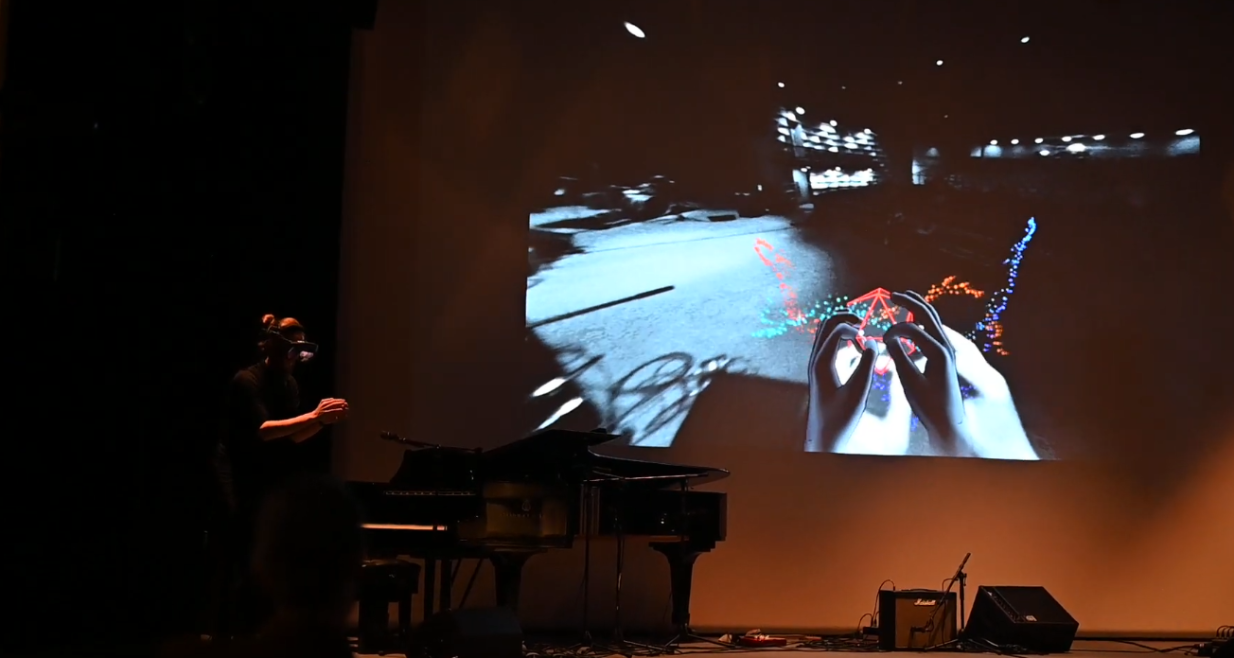
\includegraphics[height=4cm]{10-appendix-c/media/polygons-acca.png}}
    \hspace*{2cm}
    \subcaptionbox{\rurl{youtu.be/9IErsDvhXjM}}[.3\linewidth]{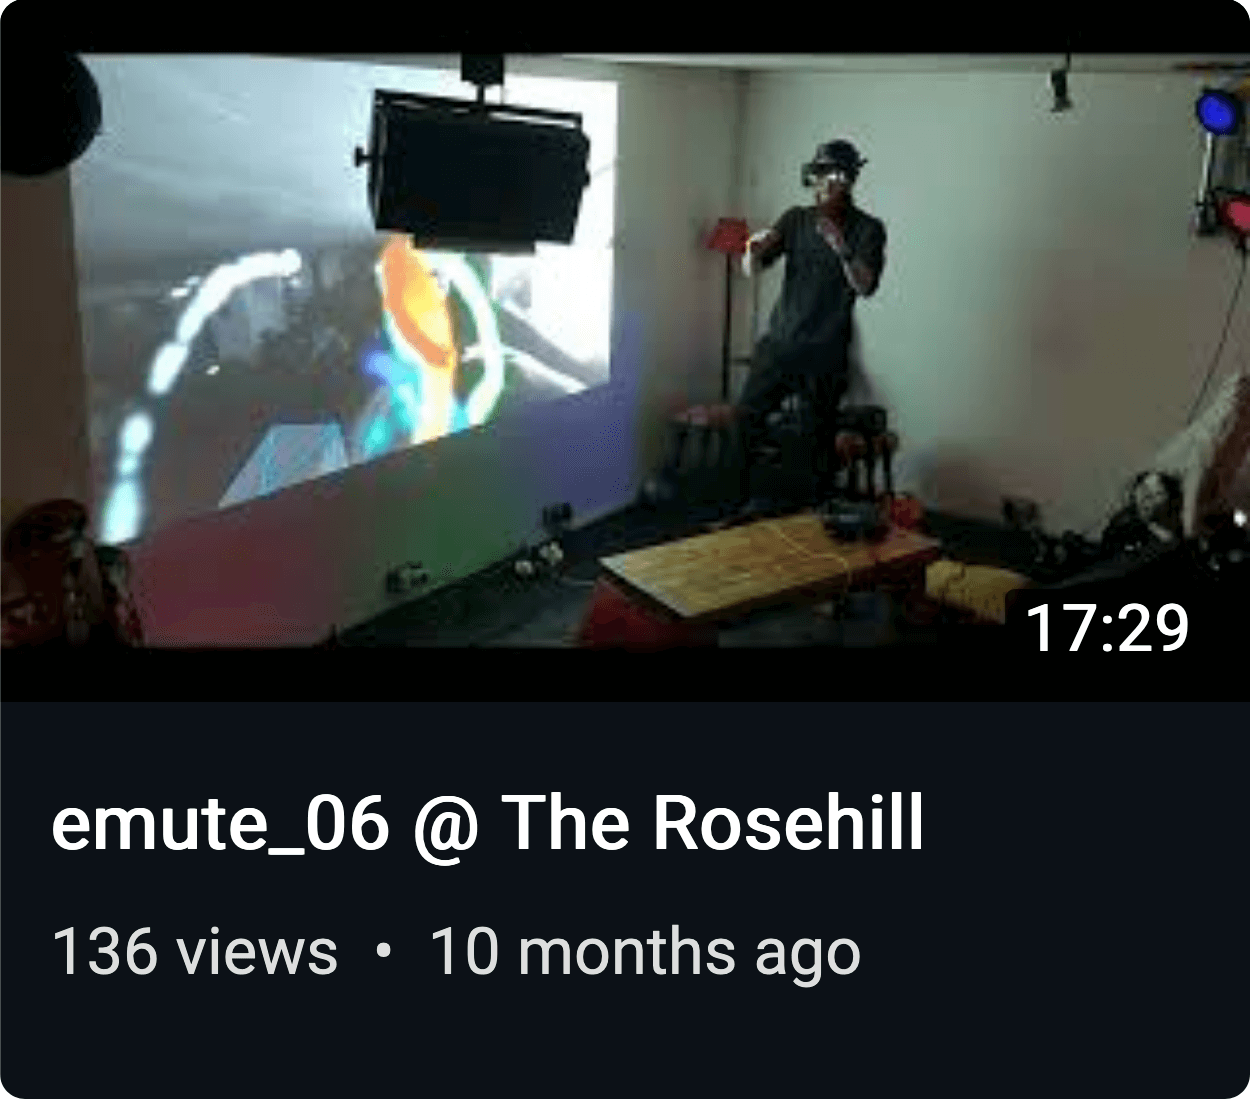
\includegraphics[height=4cm]{10-appendix-c/media/polygons-rosehill.png}}
    \caption*{polygons\textasciitilde{} Video Recordings}
\end{figure}
\clearpage


% --------------------------------------------------------------------------- %
\section{Code Repository}
\begin{figure}[!ht]
    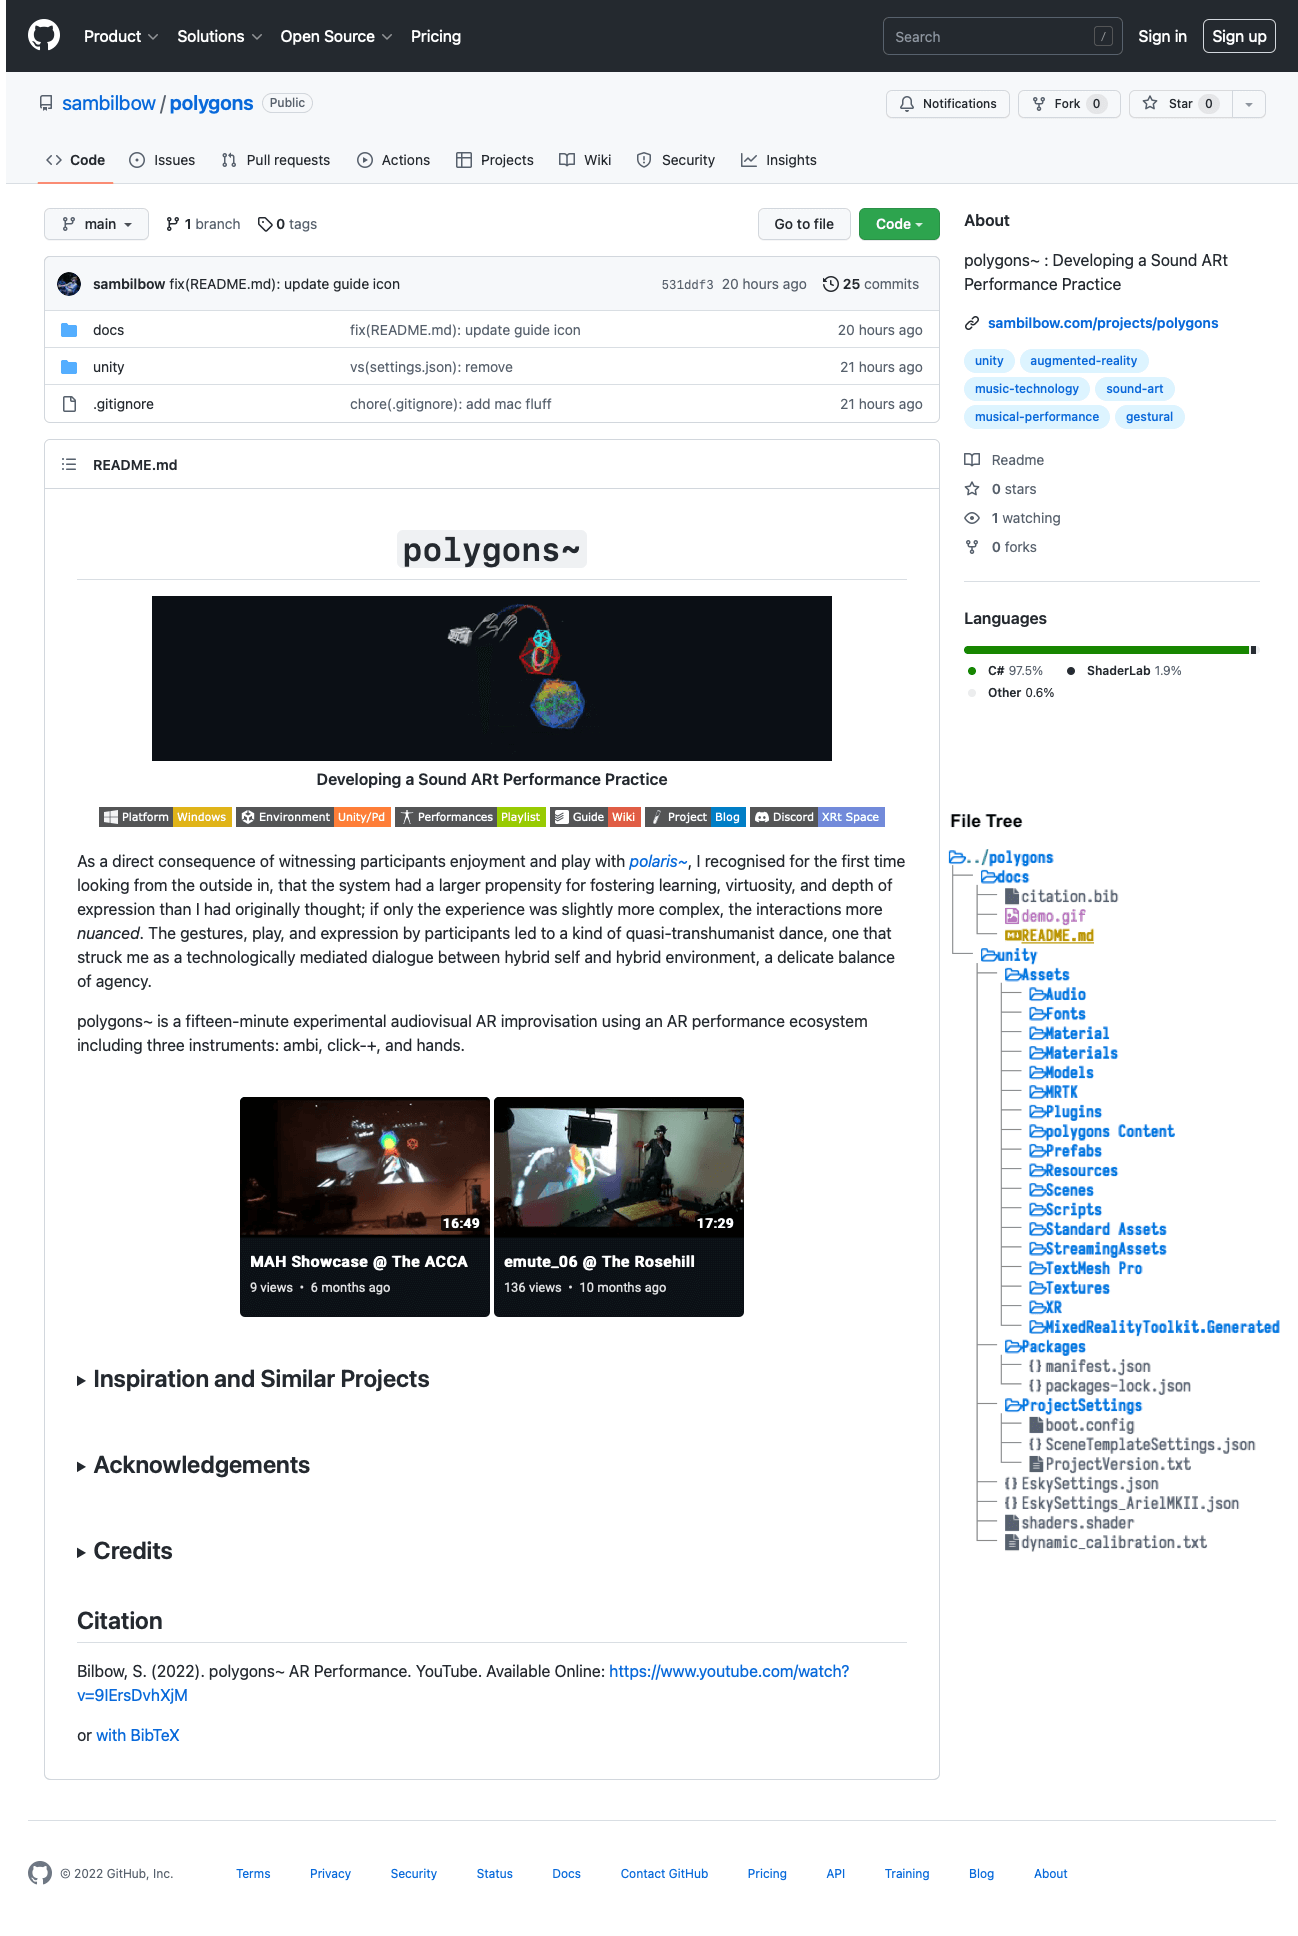
\includegraphics[width=\textwidth,height=0.9\textheight,keepaspectratio]{10-appendix-c/polygons-code-file.png}
    \caption*{\rurl{github.com/sambilbow/polygons} \\ polygons\textasciitilde{} on GitHub with file tree}
\end{figure}
\clearpage


% --------------------------------------------------------------------------- %
% \section{Blog Contents}

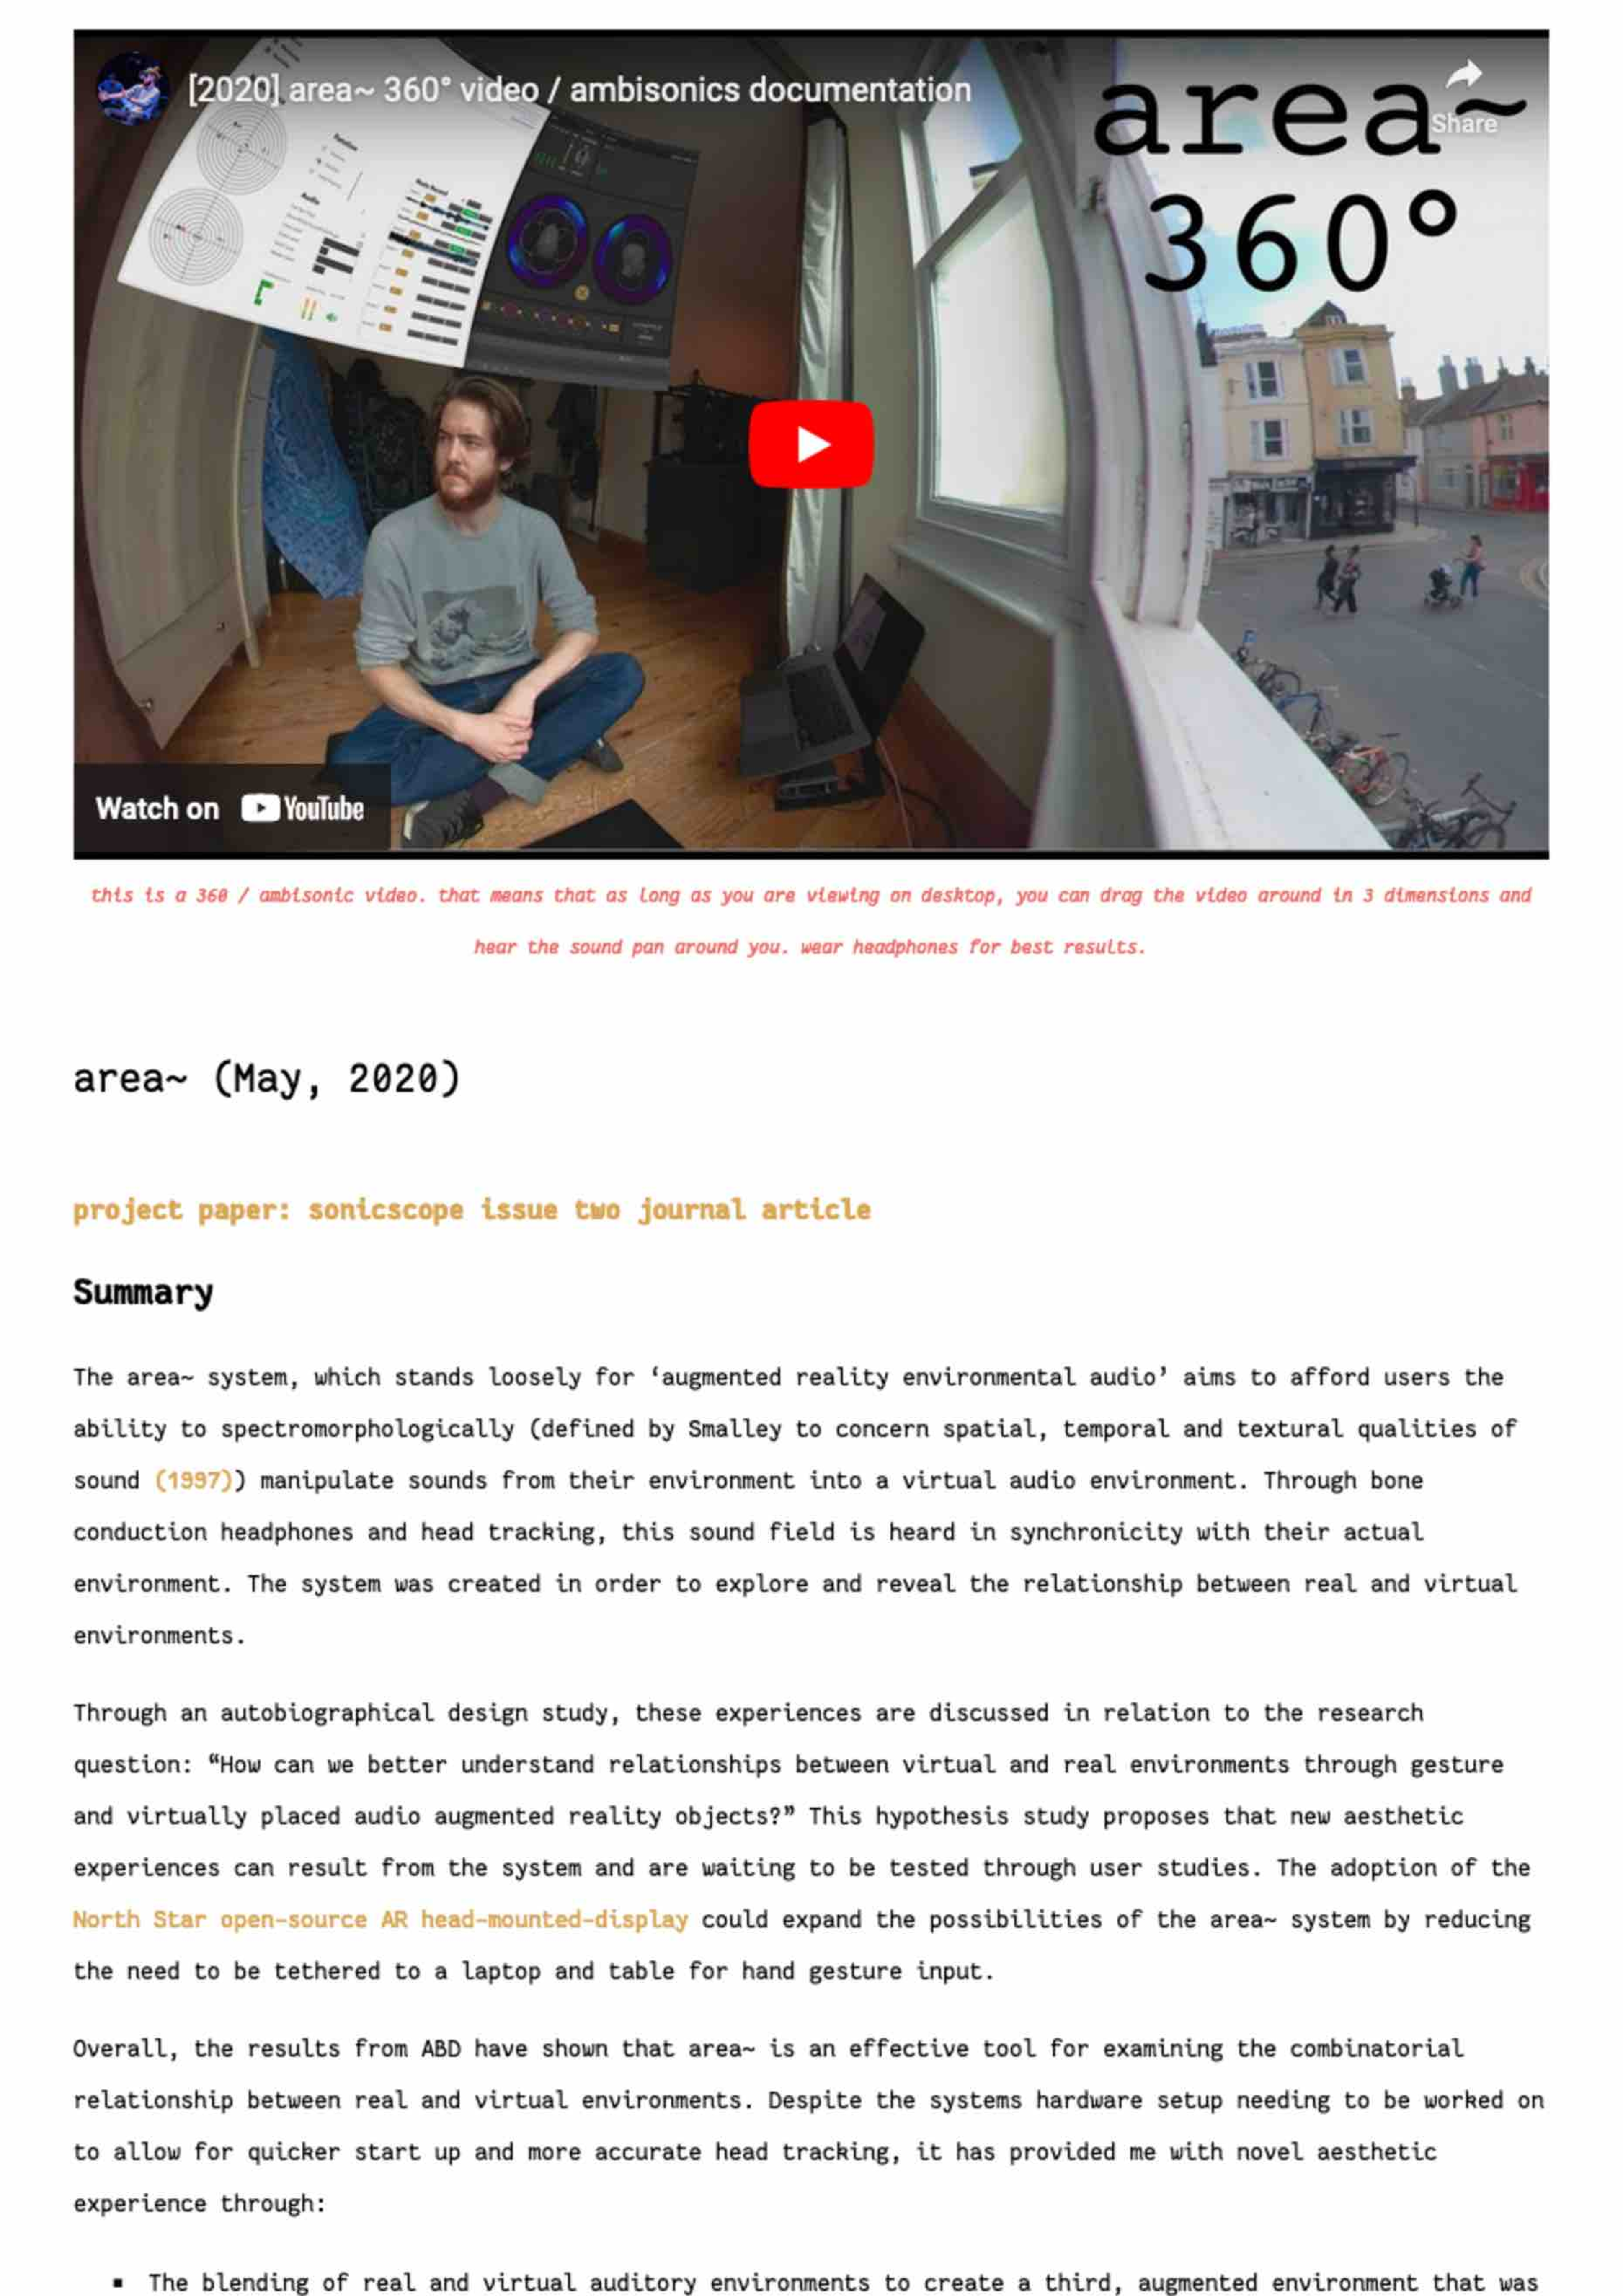
\includepdf[pages=1,pagecommand={\section{Blog Contents} \subsection{Summary}}, scale=0.71, frame, offset=10mm 0]{10-appendix-c/blog/summary.pdf}
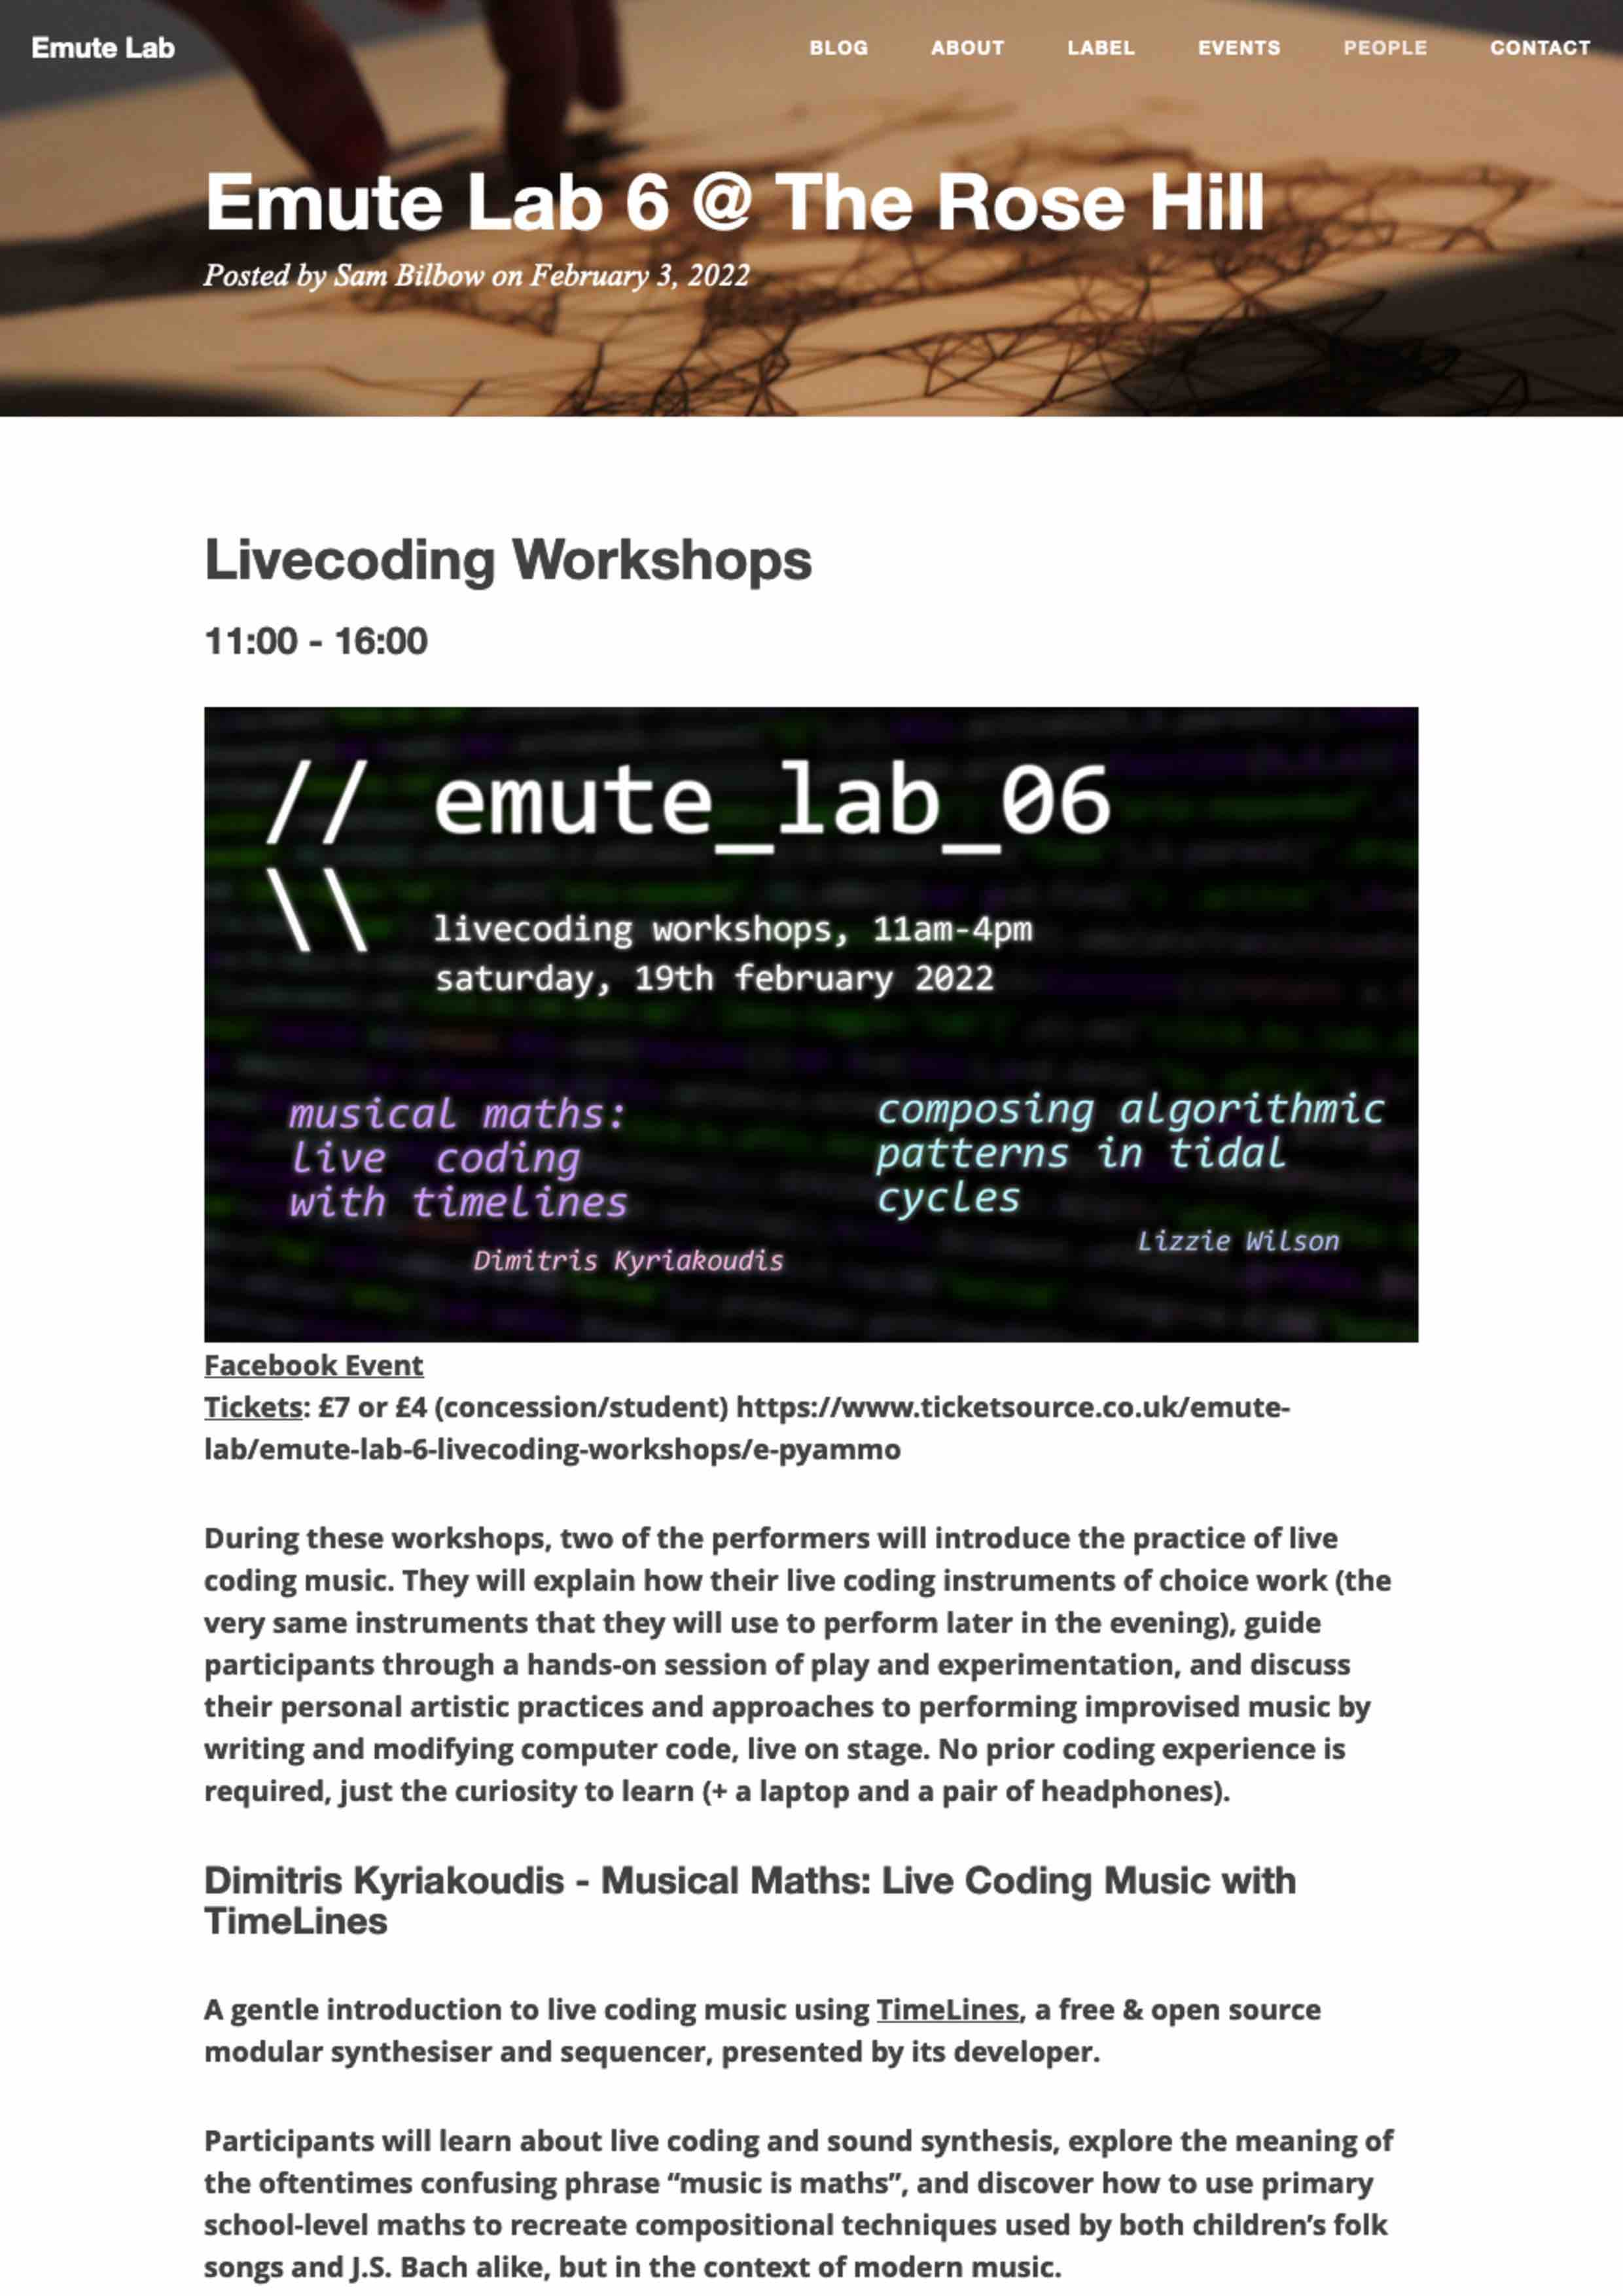
\includepdf[pages=1,pagecommand={\subsection{emute Lab Blog}}, scale=0.71, frame, offset=10mm 0]{10-appendix-c/blog/emute-blog.pdf}
\includepdf[pages=2-,pagecommand={}, scale=0.71, frame, offset=10mm 0]{10-appendix-c/blog/emute-blog.pdf}



% --------------------------------------------------------------------------- %
% \section{Project Guide}
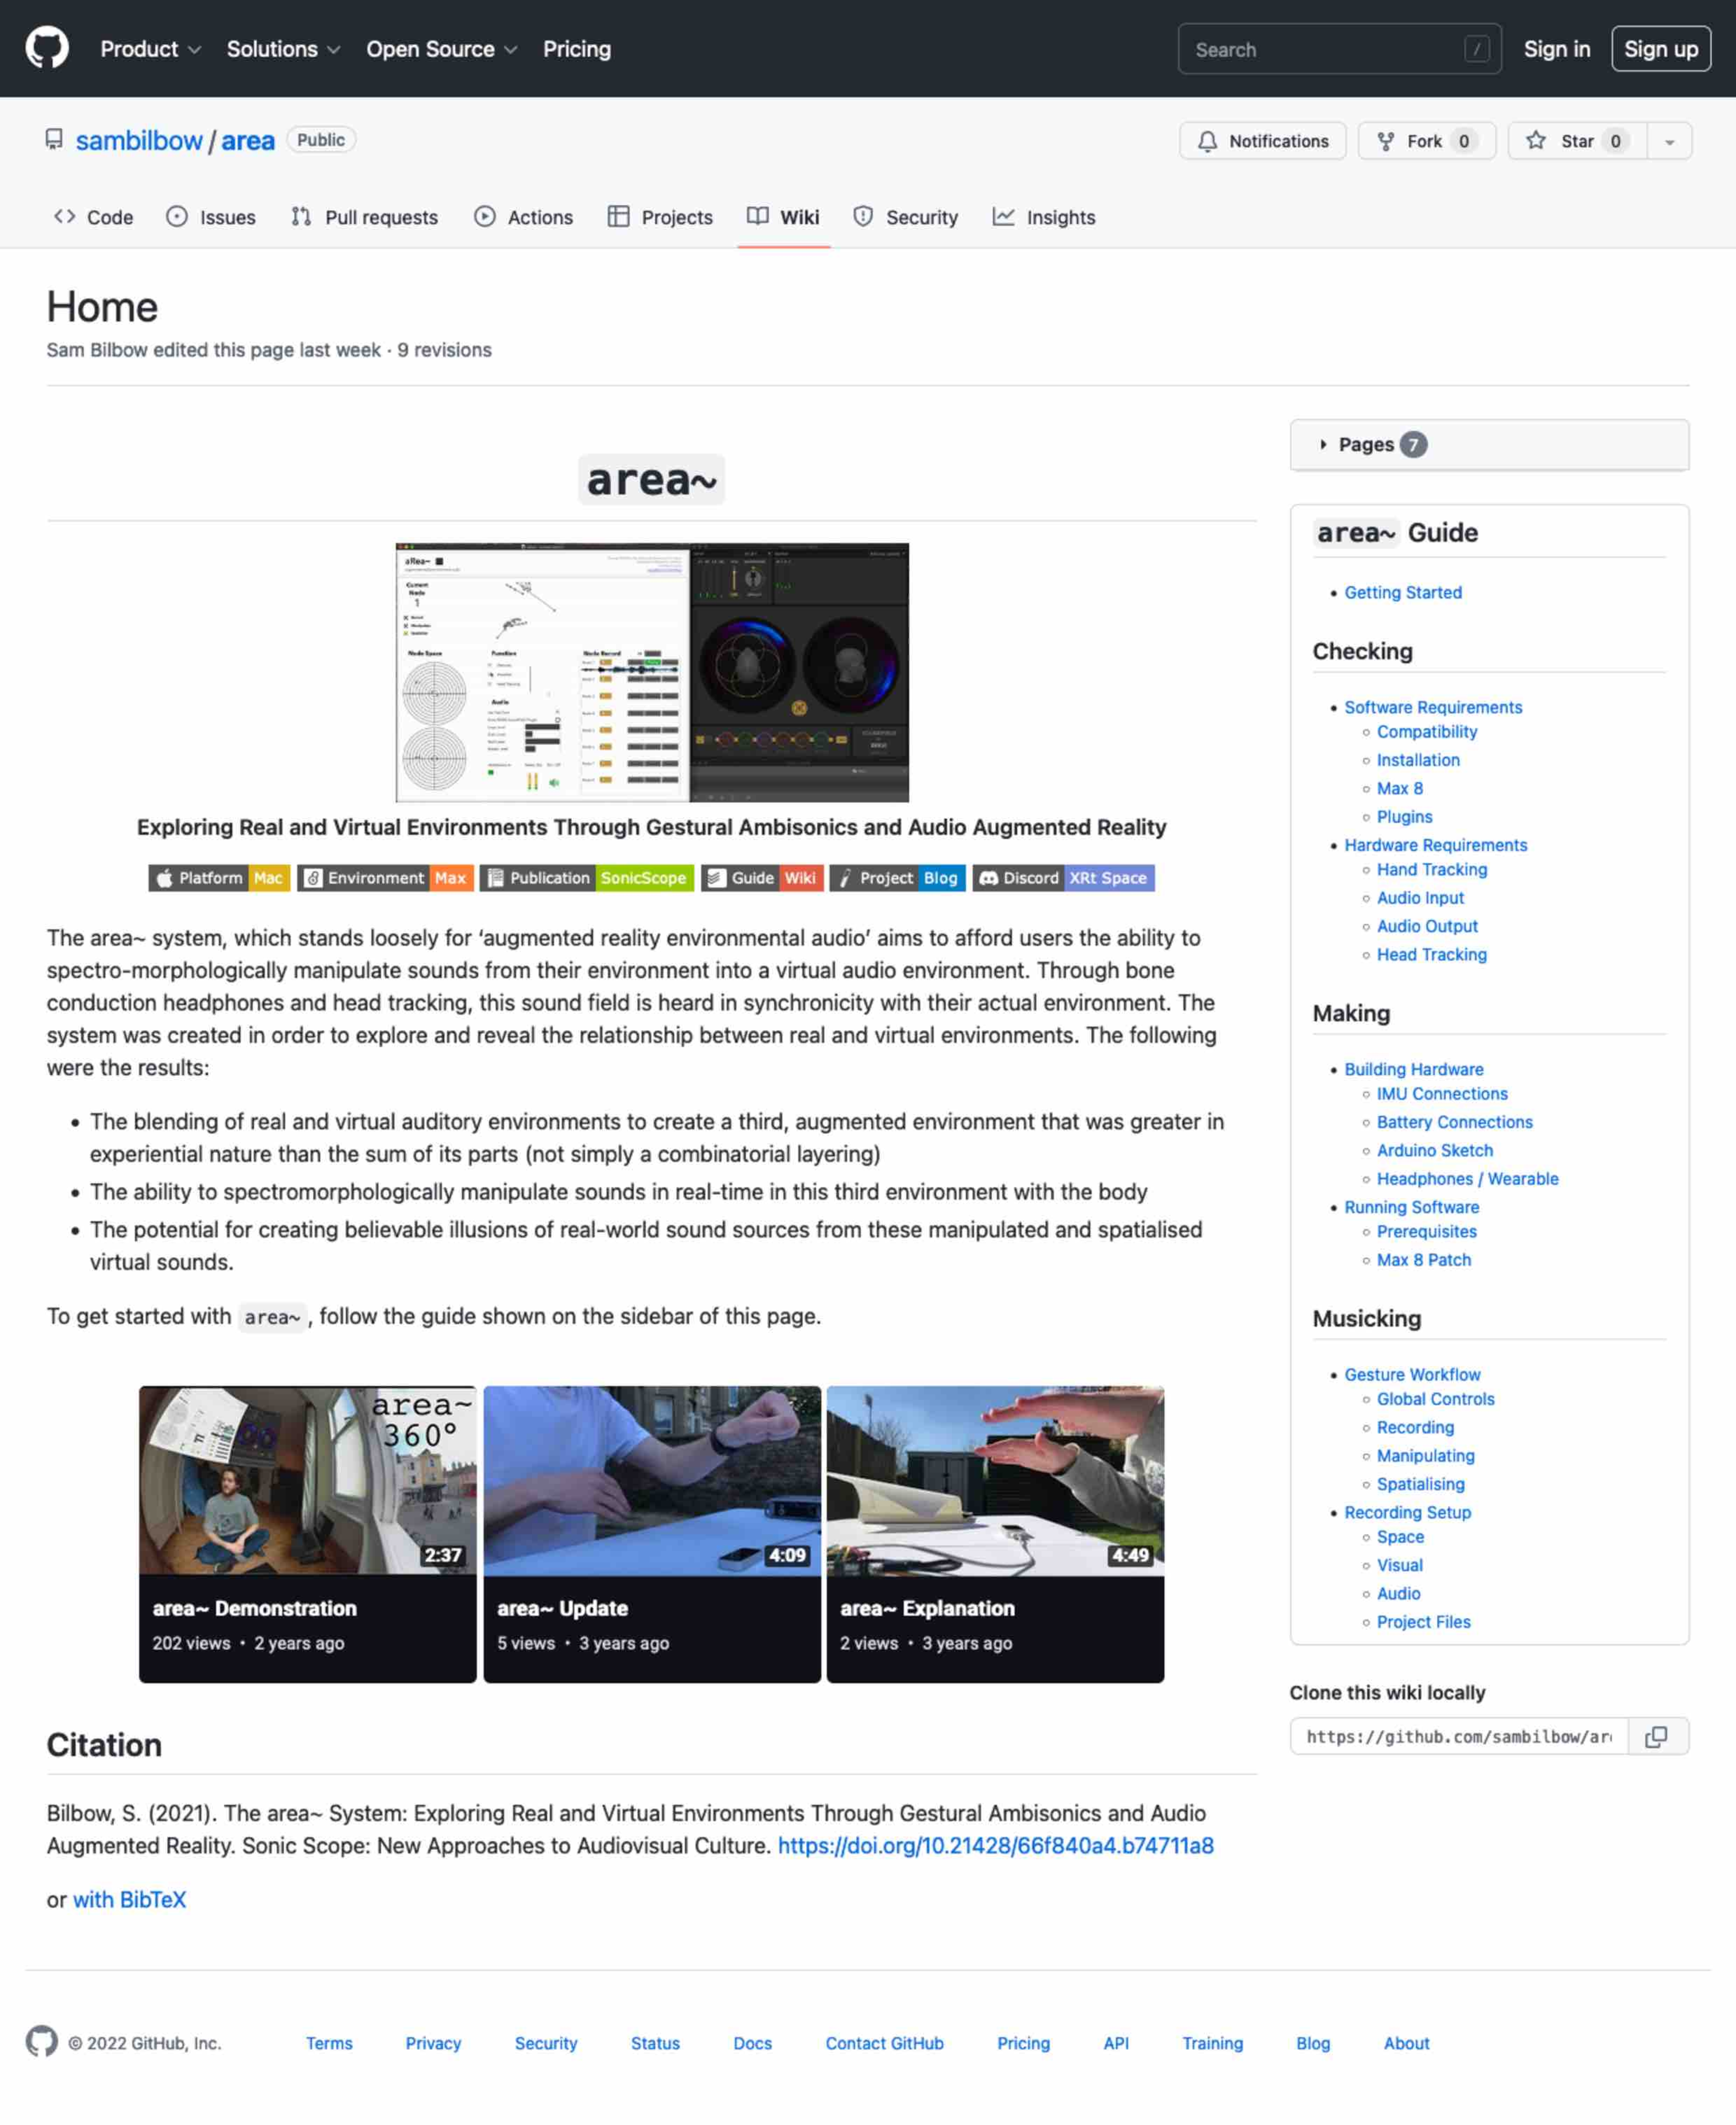
\includepdf[pages=1,pagecommand={\section{Project Guide}}, scale=0.71, frame, offset=10mm 0]{10-appendix-c/guide.pdf}
\includepdf[pages=2-,pagecommand={}, scale=0.71, frame, offset=10mm 0]{10-appendix-c/guide.pdf}